\section{Software Design}\label{sec:sw_design}

Prototyping with STM32 microcontrollers is facilitated by the STM32Cube project, which aims to simplify development by providing a comprehensive embedded software platform for each STM32 series. This software kit is complemented by the STM32CubeMX tool~\cite{cubemx}, which enables the graphical configuration of the peripherals and the clock tree of the microcontroller, as well as the automatic generation of the corresponding initialization code in the C language.

Given the opportunity to gain a deeper understanding of the tools involved in the cross-platform build process, but also to achieve greater control and flexibility over the firmware architecture, the software project is structured from scratch using CMake, without relying on STM32CubeMX. The details of the buildsystem are discussed in~\cref{subsec:buildsys}.

To benefit from the object-oriented and generic programming paradigms, the firmware is developed in \cpp. The software architecture follows a bare metal yet layered design, with a clear separation between virtualized hardware resources and application logic. Depending on the resource, the virtualization is implemented in one of two ways:
\begin{itemize}
    \item As an object, with public methods directly invoked by the application. 
    \item As a file, manipulated through I/O library functions or system calls.  
\end{itemize}
This latter approach is typical of UNIX-like systems, where special files are interfaces to device drivers, and the \ac{vfs} makes the association between the low-level operations invoked internally by file-related system calls and their implementation in the drivers. Accordingly, the firmware includes a custom implementation of a minimal virtual file system, which is presented in~\cref{subsec:files}. The device drivers and the simpler objects abstracting hardware resources are covered in~\cref{subsec:vdev}.

The firmware also relies on the following generic abstraction layers:
\begin{itemize}
    \item The \acsu{cmsis} Core(M) component, which provides a standardized API for all Arm Cortex-M processor cores. It consists of two complementary parts:
    \begin{itemize}
        \item The Core(M) Standard, delivered as a set of vendor-independent C header files directly by Arm. It declares the core exception vectors and defines the functions for accessing core and core peripheral registers, special CPU instructions, and the SIMD instructions.

        \item The Core(M) device, developed by the silicon vendor, in this case, STMicroelectronics. It declares interrupt vectors and defines the functions for startup and system configuration.

        Note that the startup assembly code provided by STMicroelectronics is not used in this project; it is replaced by a \cpp version tailored to a custom linker script.
    \end{itemize}

    \item The STM32Cube \ac{ll} drivers~\cite{UM1725}, which offer a lightweight and portable C abstraction to operate directly on memory-mapped peripheral registers. Whenever convenient, this abstraction is extended in the project with utility functions at the same abstraction level, organized by peripheral in dedicated namespaces (e.g., \icpp{dma::}, \icpp{exti::}, \icpp{flash::}).

    \item The newlib nano and GNU standard \cpp libraries. Newlib nano is a size-optimized variant of newlib, an ANSI C standard library implementation intended for use on embedded systems; it is prebuilt and distributed with the Arm GNU Toolchain.
\end{itemize}

\subsection{The Buildsystem}\label{subsec:buildsys}

CMake acts as a meta-build tool that translates an abstract buildsystem written in the CMake language into configuration files for the native build tool of the host platform.
To support cross-compilation, CMake is told about the target platform via a toolchain file. For this project, this is found split into:
\begin{description}
    \item[\itxt{arm-none-eabi.cmake}] It provides basic configuration settings for an AArch32 bare metal target. It establishes the cross-compilation environment by automatically locating the Arm GNU Toolchain installation in the host platform and defines compiler and linker options optimized for embedded development.
    In addition, it introduces interface targets corresponding to different C/\cpp runtime variants: 
    \begin{itemize}
        \item \itxt{ARM::FreeStanding} for standalone applications which do not use the standard startup files and libraries.
        \item \itxt{ARM::NoSys} for bare metal applications to weakly link system calls with stubs that implement graceful failure.
        \item \itxt{ARM::Newlib} for linking with newlib C and GNU \cpp standard libraries.
        \item \itxt{ARM::Nano}, \itxt{ARM::Nano::FloatPrint}, \itxt{ARM::Nano::FloatScan} to refine the size-optimizations of the newlib C standard library being linked.
    \end{itemize}

    \item[\itxt{armv7em-hard-fpv4sp.cmake}] It specializes the generic configuration of AArch32 bare metal targets for the Armv7-M architecture profile, also enabling the \ac{dsp} and single-precision \ac{fp} extensions. The settings are encapsulated in the interface target \itxt{ARM::V7EM-HARD-FPV4SP}.
\end{description}

\begin{listing}
\begin{minted}{text}
MEMORY
{
  FLASH (rx)  : ORIGIN = 0x08000000, LENGTH = 16K*4 + 64K + 128K*2
  NVS   (w!x) : ORIGIN = 0x08060000, LENGTH = 128K
  RAM   (w!x) : ORIGIN = 0x20000000, LENGTH = 96K
}
\end{minted}
\caption{Location and size of the memory blocks available in the \mcu target, described in the linker command language.}
\label{lst:ld_script}
\end{listing}
    
At the top level, the \itxt{CMakeLists.txt} configures project-specific settings. It loads the toolchain file, specifies the linker script, and collects the project sources and the external libraries to link with.
The linker script is a key component of the build process, as it describes how the sections in the input object files are mapped into the output executable file, and what its memory layout is.
The \mcu microcontroller is equipped with \qty{96}{\kibi\byte} of static RAM and \qty{512}{\kibi\byte} of NOR flash memory, which is partitioned in eight erasable sectors as follows: four \qty{16}{\kibi\byte} sectors, one \qty{64}{\kibi\byte} sector, and three \qty{128}{\kibi\byte} sectors. To allow for the non-volatile retention of the movement pattern, the load script reserves a dedicated memory region matching the last \qty{128}{\kibi\byte} flash sector, as shown in~\cref{lst:ld_script}.

The linker script is also tightly connected to the startup file. On system reset, the vector table is expected at address \texttt{0x00000000}, with the stack pointer reset value in its first entry. The linker ensures that this placement is satisfied and provides the stack pointer reset value, and several other addresses referenced by the code, by means of symbol definitions. Specifically, the linker script manages all the space left in the SRAM region as a shared ascending-heap/descending-stack: the start address of the region initializes the variable used to track the top of the heap in the \icpp{_sbrk()} system call, which handles heap allocation; whereas the end address of the region is put in the first vector table entry.
Other symbols are referenced while setting up the runtime context: the \icpp{Reset_Handler()} initializes the \itxt{data} segment in the SRAM by copying from the flash, according to the addresses provided by the linker; similarly, the C/\cpp initialization code makes use of these addresses to clear the \itxt{bss} segment, and to locate the initialization and de-initialization routines.

\subsection{Virtual File System}\label{subsec:files}

In general, hiding complexity behind simple and uniform interfaces is highly desirable. In UNIX-like systems, resources are abstracted as files, allowing user applications to interact with them using the same system calls as for regular files (e.g., \icpp{open()}, \icpp{read()}, \icpp{write()}, etc.). This framework relies on the \ac{vfs}, which defines a common set of low-level operations supported by all file types. These operations are invoked internally by system calls, and dispatched to their implementation depending on the file type. In particular, for special files representing character devices, the implementation of the file operations is provided by the corresponding device driver, a C kernel module that exposes the hardware as a byte stream, hiding its actual behavior.

Given the number of peripherals behaving as character devices in the project, the firmware implements a lightweight abstraction layer to support file-related system calls. This is achieved through the \icpp{IFile} and \icpp{FileManager} classes.
\begin{description}
    \item[\icpp{class IFile}] It is the abstract base class that defines the interface to operate on files. A device driver is thus a derived class that overrides the supported operations; by default, all operations are implemented in \icpp{IFile} to return the error code \icpp{-ENOSYS}.
    
    \item[\icpp{class FileManager}] It implements relevant file system services using the data structures illustrated in~\cref{fig:fm_datastr}.
    Special files are represented as \icpp{Node} objects, namely links between a file name and a driver object. The full list of special files is specified at compile time via the file manager constructor, which forwards it to initialize the node table member, as shown in~\cref{fig:node_table}.
    The open file table tracks open files at run time. As depicted in~\cref{fig:ofile_table}, each entry of this data structure holds a pointer to a node along with state data; file descriptors index the open file table and are considered free when the corresponding entries hold no valid node pointer.
    
    \begin{figure}
      \centering
      \subfloat[][Compile-time table of nodes: each entry links the name of the file representing a character device to its corresponding driver.\label{fig:node_table}]{
        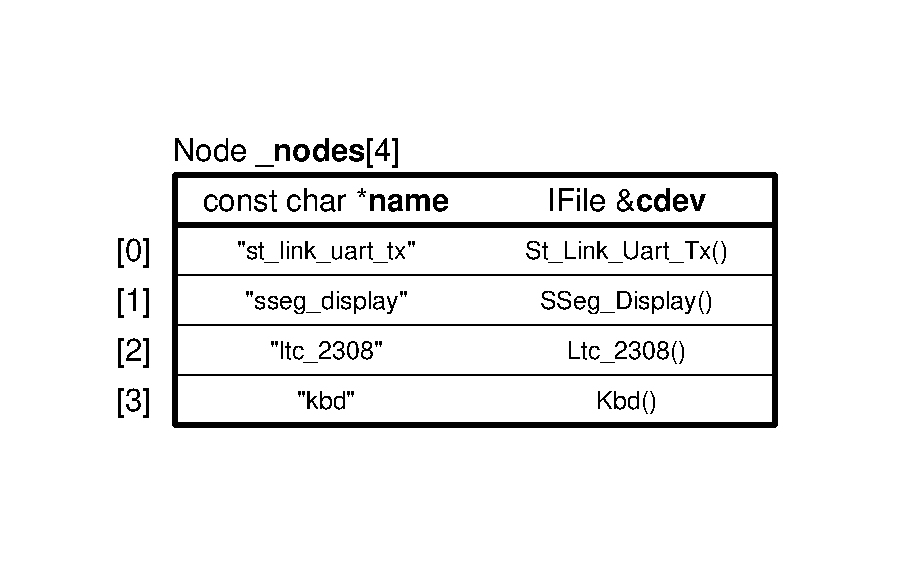
\includegraphics[width=0.45\linewidth]{../gfx/NodeTable.eps}
      }
      \qquad
      \subfloat[][Run-time table of open files, indexed by file descriptors: an open file entry holds a pointer to the associated node and some state data.\label{fig:ofile_table}]{
        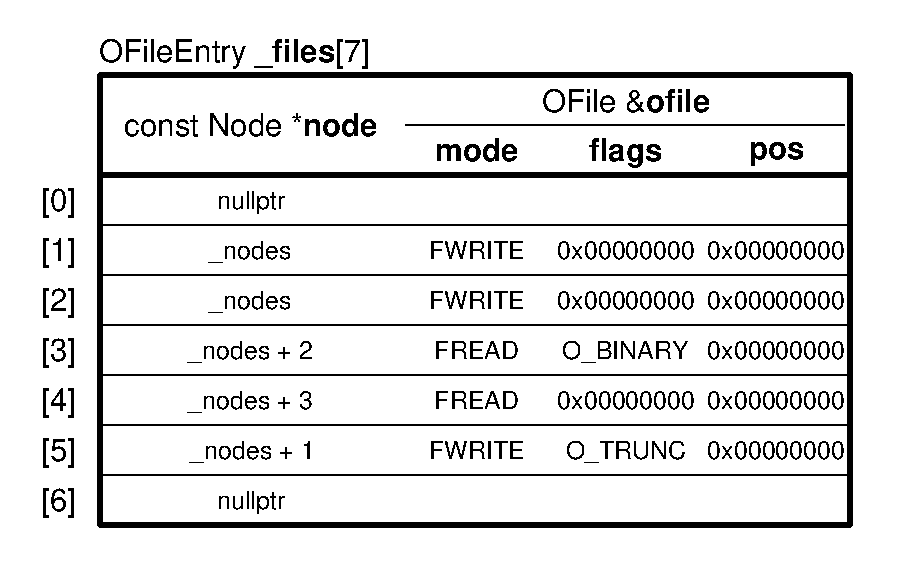
\includegraphics[width=0.45\linewidth]{../gfx/OFileTable.eps}
      }
      \caption{\icpp{FileManager} data members}
      \label{fig:fm_datastr}
    \end{figure}
    
    The file system services roughly follow POSIX semantics:
    \begin{itemize}
        \item \icpp{open()} performs name resolution through the node table to locate the associated node object. It then allocates the lowest, non-reserved file descriptor shown free in the open file table and initializes the corresponding open file table entry with the address of the node, as well as the access mode and the flags passed as arguments. Finally, the driver implementation of the operation is invoked via the node object.

        \item \icpp{close()} reverses the actions of \icpp{open()}, provided that the file descriptor identifies an open file. The driver implementation of the operation is invoked via the node pointer, which is retrieved in the open file table entry indexed by the file descriptor. Afterward, the file descriptor is released by invalidating the node pointer.

        \item \icpp{lseek()}, \icpp{read()}, and \icpp{write()} follow a similar pattern: if the file descriptor refers to an open file, the corresponding driver operation is invoked via the node pointer from the open file table.
        The only exception is that \icpp{read()} and \icpp{write()} check that the access mode specified when opening the file is compatible with the requested operation.

        \item \icpp{select()} enables monitoring multiple file descriptors for readiness to perform an I/O operation without blocking.
        Internally, for each monitored file descriptor referring to an open file, the ready state is questioned with the driver \icpp{poll()} operation, invoked via the node pointer from the open file table.
    \end{itemize}
\end{description}

\subsection{Virtualized Resources}\label{subsec:vdev}

The firmware follows two approaches when dealing with hardware resources:
\begin{itemize}
    \item Behavior close to microcontroller peripherals capabilities is abstracted through \cpp classes that directly expose a convenient interface of public member functions to the application code. This is discussed in~\cref{ssubsec:obj}.
    
    \item Behavior of complex hardware devices that fit a byte-stream access model is abstracted through device drivers, relying on the virtual file system layer.
    Note that, in all cases, device parameters are not manipulated through \icpp{ioctl()} calls, but directly with the methods exposed by the drivers.
    The device drivers are presented in~\cref{ssubsec:cdev}.
\end{itemize}

\subsubsection{Object Abstractions}\label{ssubsec:obj}

\paragraph{\mintinline[fontsize=\normalsize]{cpp}{class HwAlarm}}
It transforms a free-running general-purpose timer into an interrupt-based alarm scheduler and a delay generator.

The class is parameterized with the timer base address, allowing to refine its implementation at compile-time, based on the features of the chosen timer: namely, the width of the counter, and the number of independent capture/compare channels.
The channels are abstracted as an array of \icpp{Alarm} objects, which hold the parameters representing a runnable alarm on the corresponding channel. The representation consists of: a pointer to a callback functor, which differentiates between running alarms when valid and free channels; the remaining number of repetitions, and the periodicity converted to counter ticks.
Note that the implementation relies on the \icpp{ICallback} abstract base class to provide an interface to non-owning functor wrappers of function and member function pointers.

The setup is performed by the \icpp{init()} method. It computes the prescaler to achieve the desired counter clock resolution, then it enables the interrupt request in the \ac{nvic}, and the timer in free-running mode.

When the \icpp{setAlarm()} method is invoked to set up a new alarm, the caller specifies how many times it will fire, the periodicity, and the callback functor. Provided that there are free channels and that the periodicity is representable in the counter width, a free \icpp{Alarm} entry is initialized with the alarm parameters. The target compare value is computed starting from the current counter tick and is used to configure the corresponding capture/compare channel for interrupt generation on match events. When the interrupt fires and the handler starts executing, the triggered alarms are identified, their representation is updated, and lastly their callback functors are invoked for execution.

The \icpp{delay()} method provides traditional blocking delays, capable of exceeding the counter reload period. This is implemented through a polling loop that accumulates the elapsed time since function invocation, and compares it against the target delay.

\paragraph{\mintinline[fontsize=\normalsize]{cpp}{class PushButton}}
It implements an interrupt-based push button handler, with debouncing logic and short/long press detection.

\begin{figure}
    \centering
    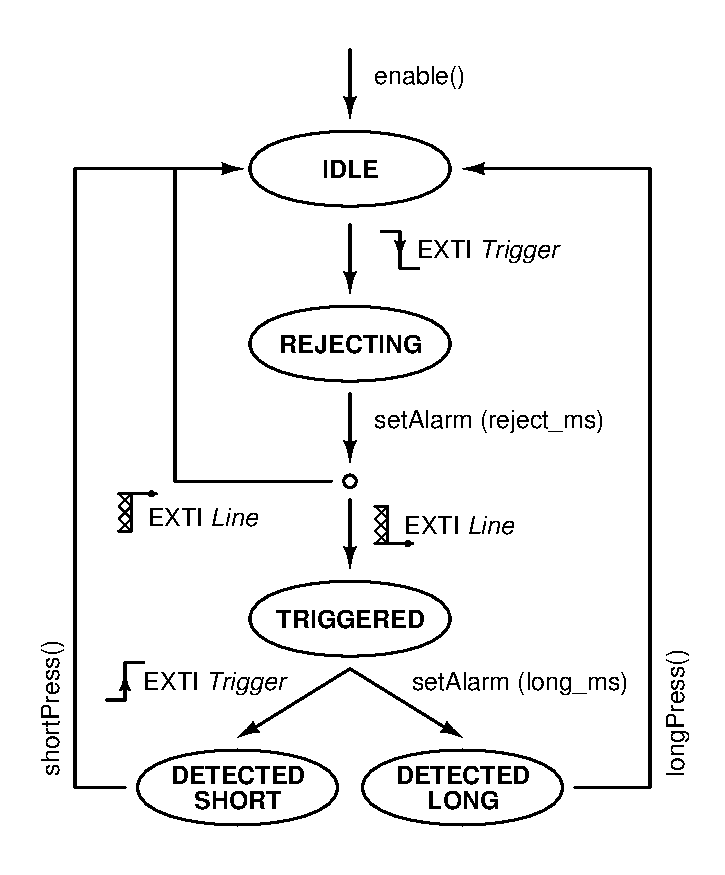
\includegraphics[width=.45\linewidth]{../gfx/PushButton_fsm.eps}
    \caption{\icpp{PushButton} internal FSM for an active low push button}
    \label{fig:pb_fsm}
\end{figure}

The class behavior follows the FSM illustrated in~\cref{fig:pb_fsm}, where the key state transitions are driven either by external edge-sensitive interrupts or by alarm timeouts. 
The application is supposed to query the button state with the \icpp{shortPress()} and \icpp{longPress()} methods, which are non-blocking and return \icpp{true} when the corresponding gesture is detected.

\paragraph{\mintinline[fontsize=\normalsize]{cpp}{class BStepper}}
It generates the waveforms required to drive the windings terminals of a bipolar stepper motor, supporting both full-step and half-step modes. This is achieved with minimal CPU overhead by delegating the transfer of precomputed bit patterns onto the GPIO port via a DMA controller, synchronized by the advanced hardware timer.

\begin{figure}
    \centering
    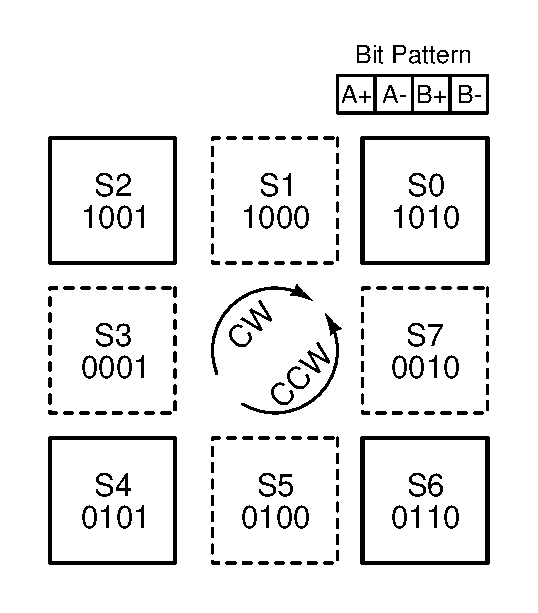
\includegraphics[width=.35\linewidth]{../gfx/Translator_states.eps}
    \caption{Bipolar motor phase states for \acs{cw} and \acs{ccw} rotations; the dashed states are skipped in full-step mode.}
    \label{fig:bsteps}
\end{figure}

Provided that the windings terminals belong to the same GPIO port, a bit pattern can be fully represented as a \ac{bsrr} mask on \qty{32}{\bit}. Given the motor phase states shown in~\cref{fig:bsteps}, the \icpp{Translator} class generates four arrays of bit patterns corresponding to \ac{cw} and \ac{ccw} driving sequences in half-step and full-step modes.
While the half-step and full-step sequences consist of eight and four states respectively, the corresponding bit pattern arrays are twice as long. This redundant data simplifies the DMA transfer, which occurs from a memory region handled as a circular buffer targeting the GPIO \ac{bsrr}. This is because the \icpp{Translator} class tracks the motor phase state as an index within the half-step sequence, ranging from \numrange{0}{7}. Without this redundancy, locating the start address of the circular buffer by simply indexing the masks arrays with a state number for half-step movements, and half that value for full-step movements, could result in out-of-bounds accesses.

The initializations of GPIO pins, DMA controller, advanced timer, and \ac{nvic} are performed by the \icpp{init()} method. The advanced timer is configured in up-counting mode, with overflows as the only source of \acp{uev}.

Motor movements are initiated with the \icpp{rotate()} method and require no further intervention from the CPU, except when the number of steps minus one does not fit in the \ac{rcr} of the advanced timer.
As a preliminary step, the \icpp{calcTimeBase()} method determines the values for the prescaler and auto-reload registers, such that the reload period matches the step duration, and the counter resolution is numerically lowest. That is
\[
    \pqty*{\text{PSC}+1}\,\pqty*{\text{ARR}+1} = \nint*{{f_\text{PSC}}\;T_\text{s}}
\]
where the step duration $T_\text{s}$ is expressed as
\[
    T_\text{s} = \frac{\qty{60}{\s\per\minute}}{N\;\omega_\text{rpm}}
\]
with $N$ being the motor resolution in steps per revolution, and $\omega_{\text{rpm}}$ the rotational frequency in revolutions per minute.

\begin{figure}
    \centering
    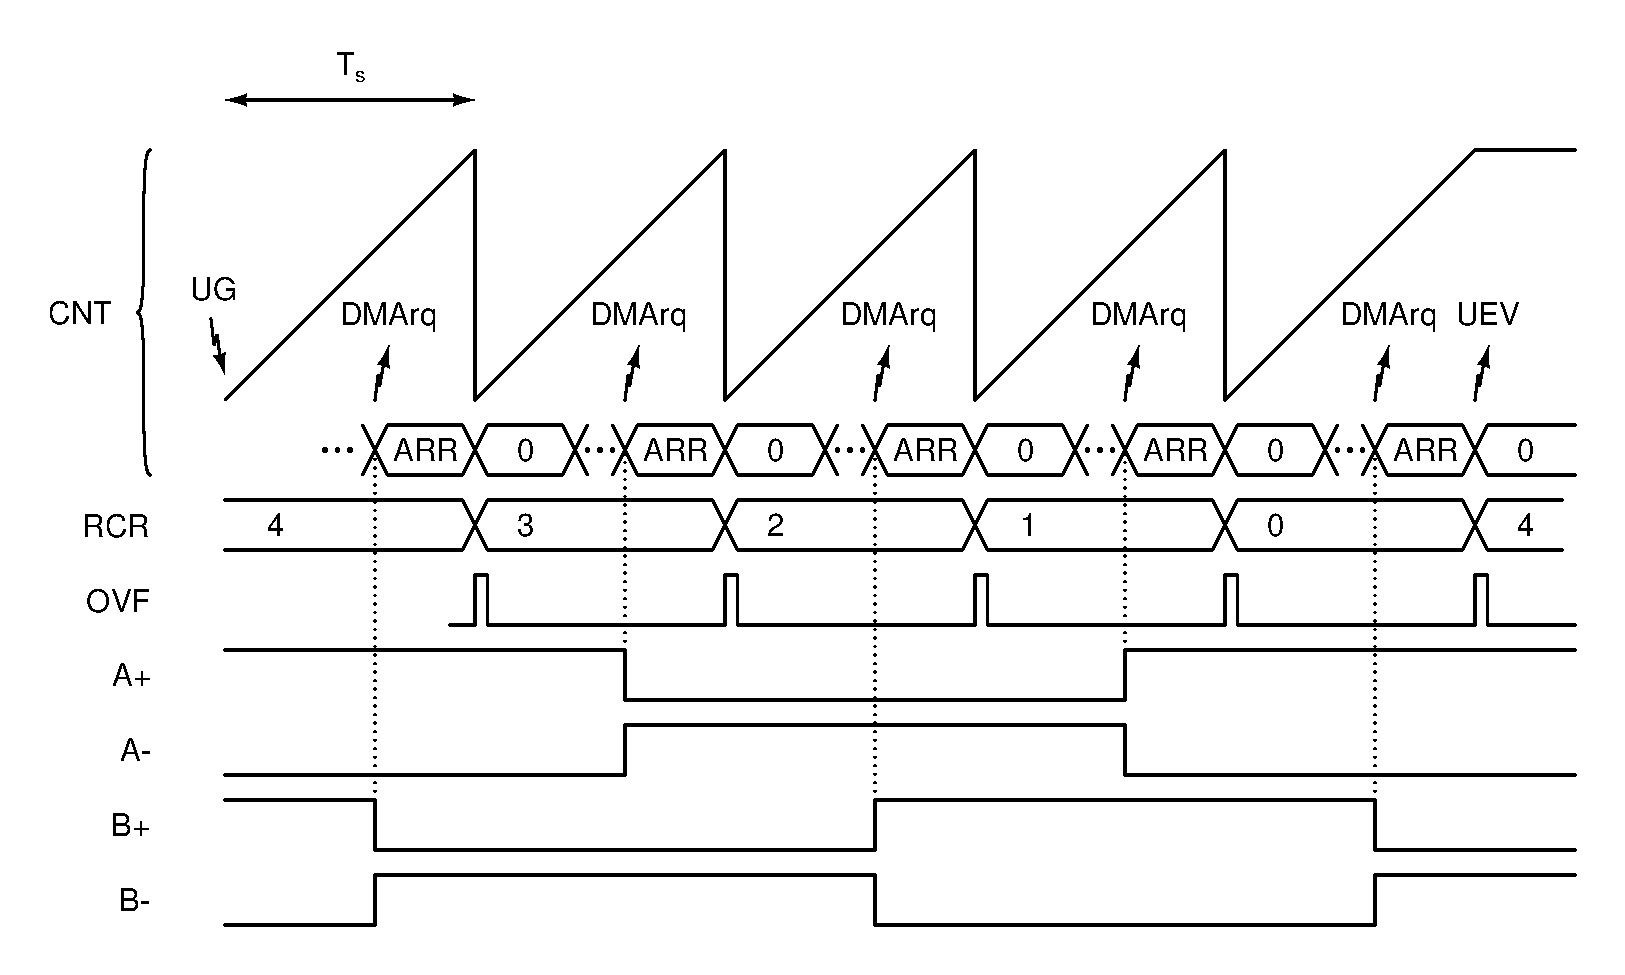
\includegraphics[width=\linewidth]{../gfx/BStepper_run.eps}
    \caption{\icpp{BStepper::rotate()} execution diagram for the simpler case when the number of steps fits the \acs{rcr}. Starting from the motor phase state S0, the motor takes five full steps in \acs{ccw} direction.}
    \label{fig:bstep_run}
\end{figure}

Considering the simpler case when the number of steps minus one fits the \ac{rcr}, the core logic is the following.
The \ac{rcr} is forcefully loaded with a software \ac{uev} and the counter is configured in one pulse mode.
The \icpp{Translator::advance()} method updates the internal motor phase state to reflect the one at the end of the movement. In addition, it locates the start address of the circular buffer with the precomputed sequence of \ac{bsrr} masks, which is used to reconfigure the DMA stream source. The last configuration step determines when to generate the DMA requests: one capture/compare channel of the advanced timer is configured to fire the requests on match events, with a compare value equal to the auto-reload register. Finally, the counter is enabled: as an example of the resulting execution diagram, see~\cref{fig:bstep_run}. 

If this approach is not feasible, the \ac{rcr} is set to its maximum value and the hardware-counted repetitions are supplemented with software-counted ones (namely, \ac{rcr} reload events). Except for the corner case where exactly one software repetition must be counted, this is handled by starting the advance timer with the one pulse mode disabled. It is configured such that, upon counter overflow and \ac{rcr} reload, the \ac{uev} generates an interrupt. The handler then updates the software repetitions count and, in the last software-counted cycle, either preloads the \ac{rcr} or directly switches the counter to one pulse mode. In the former case, at the end of the software repetitions count, the counter is switched to one pulse mode as well.

\paragraph{\mintinline[fontsize=\normalsize]{cpp}{class MotionPattern}}

It implements an \icpp{std::vector}-like container for \icpp{MotionSegment} objects, that is allocated in a flash sector with wear-levelling and cached in SRAM over a statically allocated array.

The class is parameterized by the maximum number of elements it can contain.
While the elements stored in the SRAM array are plain \icpp{MotionSegment} objects, the corresponding flash entries are instances of a larger type, \icpp{FlashChunkEntry}, which packs an additional byte attribute that indicates whether the entry is valid (\icpp{WRITTEN = 0xAA}) or not (\icpp{ERASED = 0xFF}).

As it happens in the application, suppose that the class allocates the non-volatile container in the \qty{128}{\kibi\byte} sector starting at address \texttt{0x08060000} and that the \icpp{FlashChunkEntry} is represented on \qty{8}{\byte}. If the maximum number of elements is taken to be four, then the sector can accomodate
\[
    N = \frac{\qty{128}{\kibi\byte}}{\text{\icpp{sizeof(FlashChunkEntry[4])}}} = 4096
\]
distinct containers, hence the logical partitioning of the sector into corresponding $N$ chunks. The wear-levelling mechanism leverages this excess space to minimize the number of sector erasures. Clearing the non-volatile container does not immediately cause a sector erase; instead, it invalidates the current chunk and enables the next one available. This process continues until all chunks have been invalidated, only then the sector is erased. To illustrate, consider~\cref{fig:mp}:
\begin{enumerate}[label=\textbf{(\alph*)}]
    \item Starting in the erased state, the container is located in the first chunk and has a zero size; entry zero is pointed to be the written next.
    \item After three write operations, the container is still located in the first chunk. The fourth entry is pointed to be written next.
    \item The container is cleared: the chunk is invalidated by marking the first entry as \icpp{DIRTY = 0x00}. The container is now located in the second chunk and entry zero is pointed to be written next.
    \item After $N-1$ clear operations, all chunks are marked dirty but the last one. A further clear operations triggers a sector erase.
\end{enumerate}

\begin{figure}
    \centering
    \subfloat[][Fully erased sector, empty container\label{fig:mp_ff}]{
        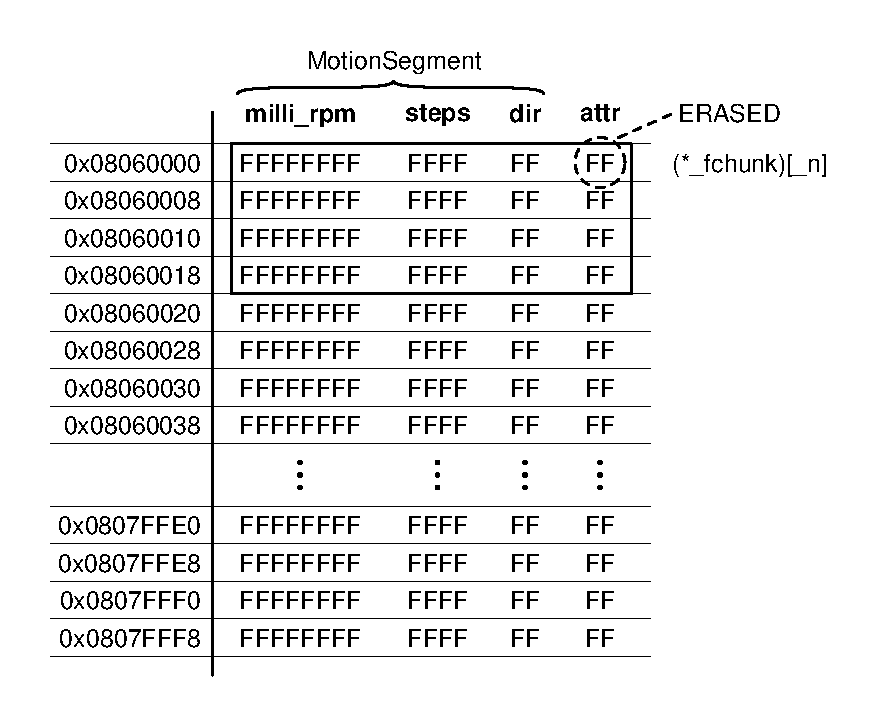
\includegraphics[width=.47\linewidth]{../gfx/MotionPattern_ERASED.eps}
    }\hfill
    \subfloat[][First chunk in use, container size is three\label{fig:mp_wr}]{
        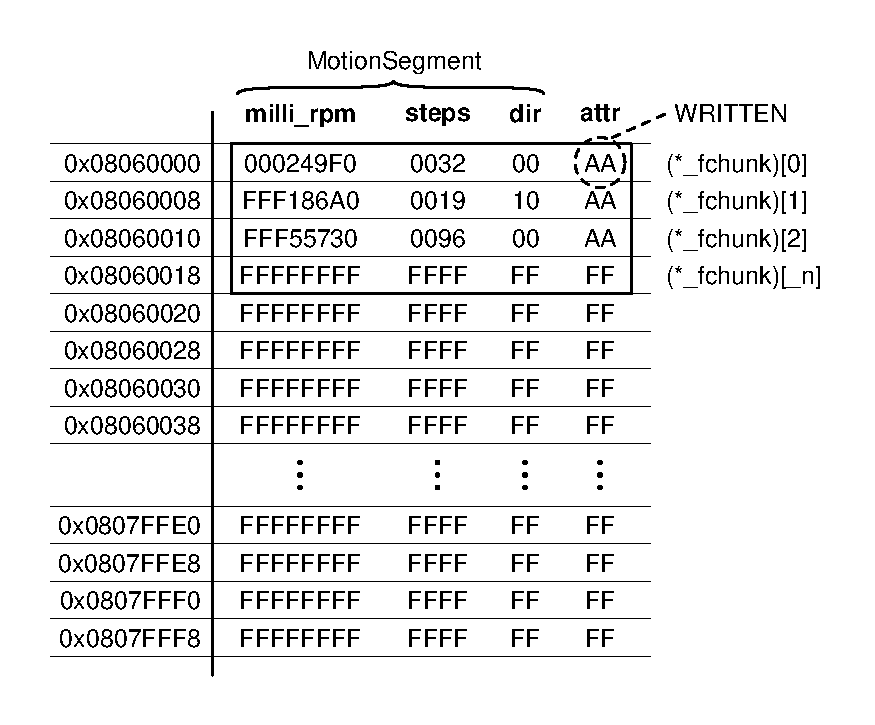
\includegraphics[width=.47\linewidth]{../gfx/MotionPattern_WRITTEN.eps}
    }\\
    \subfloat[][First chunk marked dirty, second chunk in use, container is empty\label{fig:mp_dy}]{
        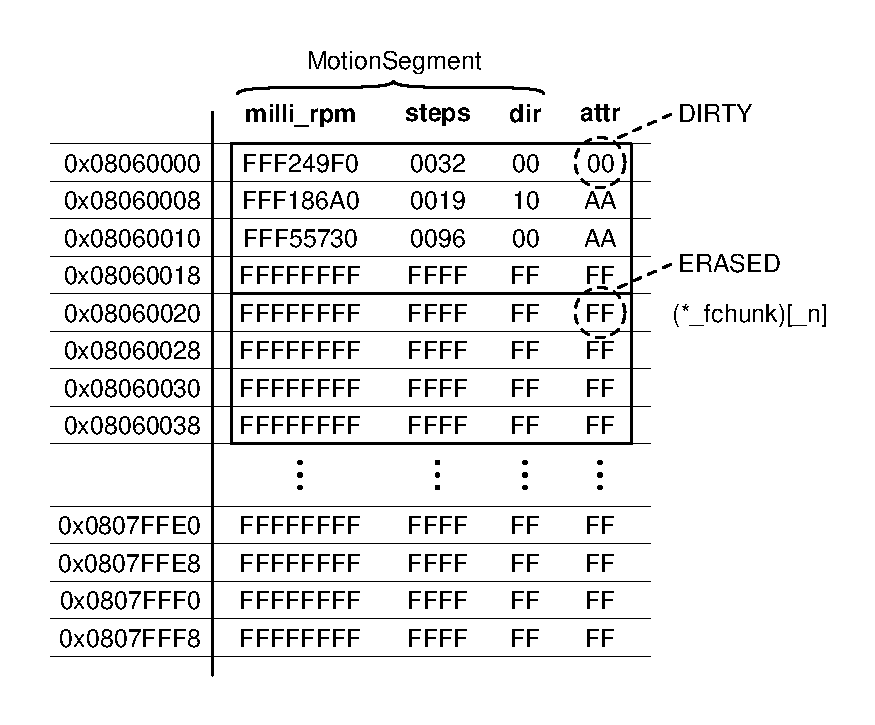
\includegraphics[width=.47\linewidth]{../gfx/MotionPattern_DIRTY.eps}
    }\hfill
    \subfloat[][All chunks marked dirty but the last one in use. Clearing the container triggers a sector erase.\label{fig:mp_te}]{
        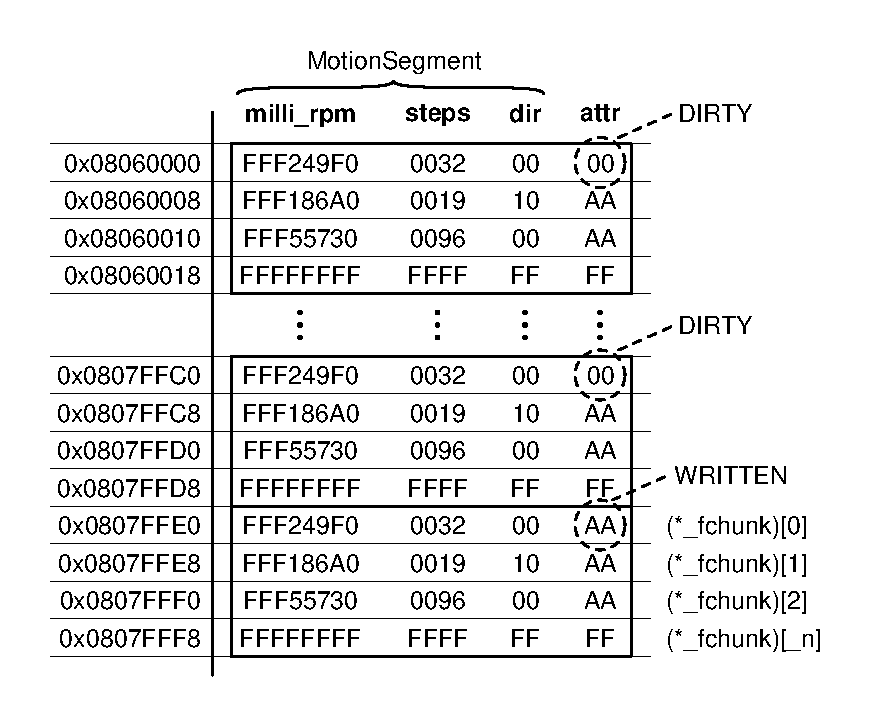
\includegraphics[width=.47\linewidth]{../gfx/MotionPattern_TOERASE.eps}
    }
    \caption{\icpp{MotionPatter} logic for managing the persistence of the \icpp{MotionSegment[4]} array.}
    \label{fig:mp}
\end{figure}

\paragraph{\mintinline[fontsize=\normalsize]{cpp}{class SpiMaster}}

It provides a simple interface to communicate with multiple SPI slave devices, internally managing the select-signal generation via GPIO.

During initialization, the GPIO pins assigned to \acsu{sclk}, \acsu{mosi}, and \acsu{miso} are configured in the alternate function corresponding to SPI. Since these pins are left floating when the controller is disabled, weak pull-downs are enabled. The SPI controller is configured as well, preparing for master-mode, full-duplex operation with software-managed slave selection.

The communication targets are abstracted as an array of \icpp{Slave} objects, each holding the protocol parameters and the GPIO pin to be used for slave selection. Targets are dynamically registered via the class interface: provided that there are free entries in the array of targets, the \icpp{addSlave()} method computes the lowest prescaler that satisfies the requested \ac{sclk} maximum frequency, and stores the SSN pin information and protocol parameters. It returns the index of the newly registered slave, which serves as its identifier. 
Although the \mcu SPI peripheral supports only \qty{8}{\bit} and \qty{16}{\bit} transfers, the class accommodates arbitrary frame lengths up to \qty{16}{\bit} by adjusting the alignment of the transmitted and received data.

Full-duplex transfers are blocking and are performed with the \icpp{txrx()} method specifying the identifier of the target slave. If the retrieved slave-dependent configuration differs from the last active one, the SPI controller is reconfigured accordingly. Note that, in this case, the configuration of weak pull-up/down resistors on \ac{sclk} is changed to match the clock polarity required by the slave. 
Then the method asserts the SSN line, generates a pre-transfer delay via the \icpp{HwAlarm} abstraction, executes the transfer, and de-asserts the SSN line after a post-transfer delay. 

\subsubsection{Device Drivers}\label{ssubsec:cdev}

\paragraph{\mintinline[fontsize=\normalsize]{cpp}{class UartTx}}

It is a lightweight driver for the USART peripheral, implementing DMA-based UART transmission in blocking or non-blocking fashion.

The driver object is configured directly through its public methods, which includes assigning a GPIO pin, a DMA stream, and protocol parameters like frame settings and baud rate. Note that the character payload has a fixed length of \qty{8}{\bit}.

The initialization of the underlying peripherals is performed when opening the device file, which supports only the write mode. The DMA stream is prepared for a memory-to-peripheral direct byte transfer: the source address points to the start of the characters buffer and is auto-incremented by the DMA controller; the destination is fixed and corresponds to the data register of the USART peripheral. On the USART side, following the configuration of the protocol parameters, the DMA transmission mode is enabled.

The implementation of the \icpp{write()} operation is trivial. If there is an ongoing transfer, the open-file flags are queried to determine if it is acceptable to block while waiting for it to complete. Upon completion, the user data buffer is copied locally, the DMA stream is enabled, and the transmission continues with no further intervention from the CPU.

\paragraph{\mintinline[fontsize=\normalsize]{cpp}{class SSegDisplay}}

It is the driver for the display peripheral presented in~\cref{subsec:sseg}, implemented by extending the generic capabilities of the \icpp{UartTx} base class with functionalities such as character re-encoding, text buffering, and interrupt-based text scrolling.

In addition to the configuration of the base driver object, the method \icpp{setDisplay()} allows to configure the number of 7-segment displays composing the peripheral screen, the minimum number of times a string that does not fit on the screen should be scrolled, and the scrolling speed.
The alphabet supported by the peripheral is built at compile time via the template function \icpp{fmtChar()} and made available for the re-encoding of an ASCII stream through the private method \icpp{encode()}.

Opening the device file performs the same initialization described for the base class, with the only peculiarity that truncation forces the driver to transmit a \icpp{CLEAR} command to the peripheral.

\begin{figure}
    \centering
    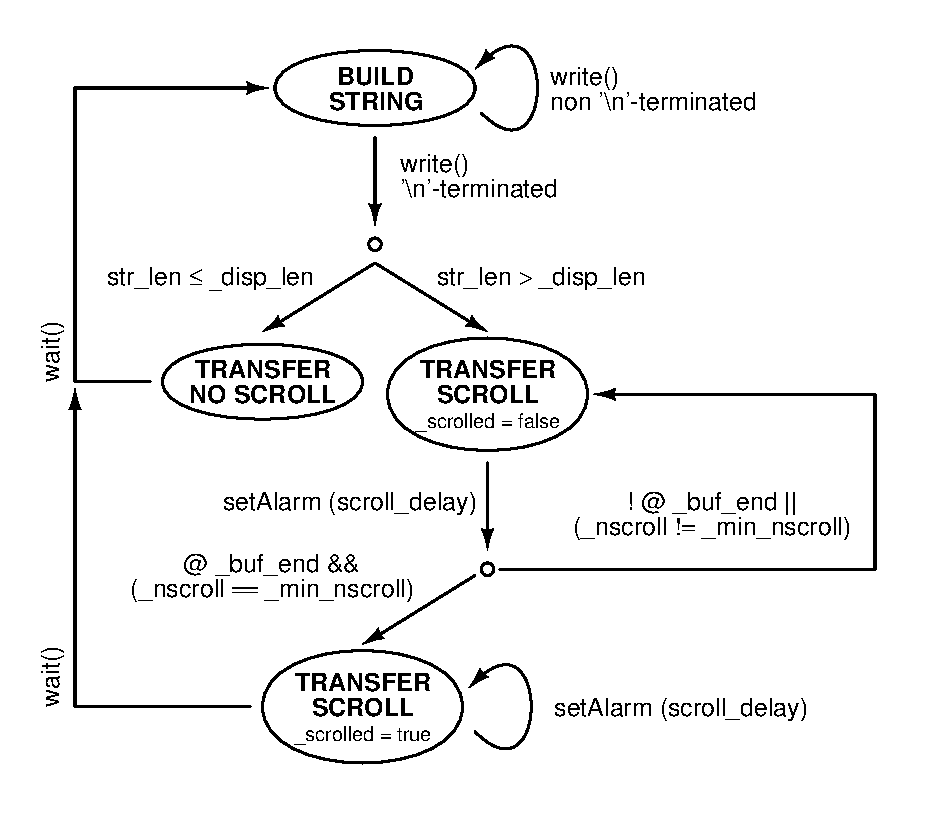
\includegraphics[width=.6\linewidth]{../gfx/SSegDisplay_fsm.eps}
    \caption{\icpp{SSegDisplay} internal FSM for text scrolling}
    \label{fig:sseg_fsm}
\end{figure}

At the core of the \icpp{write()} method there is the agreement that the newline character indicates the termination of a string to be transmitted. It is expected that the text may exceed the screen length, hence the implementation of an interrupt-based mechanism to handle the scrolling of the displayed text. This is achieved in collaboration with the \icpp{HwAlarm} class, following the FSM illustrated in~\cref{fig:sseg_fsm}, where the state transitions are driven either by application logic or by alarm timeouts.

It is worth noting that when the driver is scrolling a string, the alarm callback is executed by the \icpp{HwAlarm} object within an interrupt handler. Since the UART transfer is synchronized via DMA, the amount of processing required in CPU Handler Mode is minimal. This holds true except when the last contiguous substring has been transmitted to the peripheral, in which case a \icpp{std::rotate()} operation is performed to manipulate the underlying character buffer and produce the effect of continuous scrolling.

\paragraph{\mintinline[fontsize=\normalsize]{cpp}{class LTC2308}}

It is a full driver for the ADC peripheral discussed in~\cref{subsec:adc}, implemented according to the timing diagrams and the applications information found in the datasheet~\cite{ltc2308}.

The class collaborates with the \icpp{SpiMaster}, in charge of the low-level details of SPI communication, and with the \icpp{HwAlarm}, that generates the delays required to satisfy timing constraints.
The configuration of the driver object includes specifying the protocol-related parameters required for registering a slave with the \icpp{SpiMaster}: these are the \ac{convst} pin, which triggers both the start of the analog-to-digital conversion process and the start of the SPI transfer, and the maximum \icpp{sclk} frequency.
In addition, the \icpp{setOptions()} method internally generates the programming word that configures the actual ADC peripheral, based on the input range type (unipolar or bipolar), the input stage type (single-ended or differential), the multiplexer channels, and the power management mode.

Opening the device file has the effect of registering the slave target with the \icpp{SpiMaster} and transmitting the programming word to initialize the ADC peripheral with the selected options. 
The \icpp{read()} method implements the logic for acquiring a stream of \qty{12}{\bit} samples from the ADC peripheral and transforming it into a binary stream of \qty{16}{\bit} signed or unsigned integers, according to the selected options.

\paragraph{\mintinline[fontsize=\normalsize]{cpp}{class Keyboard}}

It is a full driver for PS/2-compatible keyboards using scan code set 2, interfaced through the custom PS/2-to-SPI peripheral described in~\cref{ssubsec:ps22spi}.

Communication with the SPI slave and timing synchronization are implemented similarly to the \icpp{LTC2308} driver, relying on the \icpp{SpiMaster} and \icpp{HwAlarm} abstractions. The \icpp{SpiMaster::txrx()} function is further abstracted with private helper methods, tailored to the behavior of the peripheral device:
\begin{description}
    \item[\icpp{_pollTxRx()}] Sends a command to the peripheral and polls for an acknowledgment within a bounded number of SPI cycles. This approach is necessary because: first, command execution requires time; second, the full-duplex nature of the transfer implies that data received from the slave cannot represent the response to the command being sent concurrently.

    \item[\icpp{_trySet()}] Builds upon \icpp{_pollTxRx()} to implement the transmission logic of the PS/2 \textit{Set/Reset Status Indicator} command to the keyboard, which consists of a command byte followed by an argument byte. First, an SPI command programs the PS/2 controller in transmit mode to send \texttt{0xED}; the controller is then reconfigured to receive the keyboard's acknowledgment. The process is repeated to transmit the argument byte.
\end{description}

Opening the device file registers the slave with the \icpp{SpiMaster} and issues a reset sequence: inside the peripheral, the PS/2 controller is disabled and re-enabled, and the FIFO buffer is flushed. Then, \icpp{_trySet()} is invoked to turn off both the Num Lock and Caps Lock indicators.

The \icpp{poll()} operation must determine whether a subsequent \icpp{read()} call would return a character, ideally without blocking. In practice, one blocking SPI transfer is performed via the helper method \icpp{_tryRead()} to check if a scan code is available for processing. Note, however, that the presence of a scan code does not guarantee that a character is ready to be returned. This is where the parsing machine comes into play. It consists of:
\begin{description}
    \item[\icpp{class ScanCodeParser}] Implements the logic for parsing the scan codes belonging to set 2 with a FSM and a lookup table. Processing any scan code generates a \icpp{ParsedKey} object, which is differently interpreted based on its \icpp{Action} field. Some scan codes merely advance the FSM without yielding actionable information; these are represented with action \icpp{NONE}. Conversely, the \icpp{MAKE} and \icpp{BREAK} actions are paired with the layout-independent representation of the key for which the make or break code has been received; this is represented as an enumerator of \icpp{UniKey} type.

    \item[\icpp{_map()}] Translates layout-independent \icpp{UniKey} keys into ASCII characters using a layout-specific lookup table, considering the current state of modifier keys (Left/Right Shift, Alt Gr, Caps Lock, and Num Lock).
    
    Note that while the current implementation provides the Italian lookup table, the mapping can be generalized through template parameters and specialization.
    
    \item [\icpp{_step()}] Overall, it implements the logic that translates scan codes into ASCII characters, returning \icpp{'\0'} when the scan code does not yield such information.

    In details, the scan code is first parsed into a \icpp{ParsedKey} object. If the action is \icpp{MAKE} or \icpp{BREAK}, the associated key is processed as follows:
    \begin{itemize}
        \item If it corresponds to a modifier key, the internal state is updated accordingly. For Caps Lock and Num Lock, a small FSM determines whether the corresponding keyboard indicators should be updated, in which case \icpp{_trySet()} is invoked.
        
        \item Otherwise, only key press (corresponding to the \icpp{MAKE} action) requires processing. In this case, the \icpp{_map()} helper function is invoked.
    \end{itemize}
\end{description}
Tying things together: if \icpp{_tryRead()} yields a scan code, it is processed by \icpp{_step()}, which may produce a non-zero character, which updates the internal \icpp{_peek} member. The \icpp{poll()} operation returns accordingly: a \icpp{_peek} value different from \icpp{'\0'} indicates read readiness.

The \icpp{read()} function complements this behavior. If \icpp{poll()} was previously called, the \icpp{_peek} value may already contain a character. If not, and the open file flags allow blocking, a character is fetched using the helper method \icpp{_getc()}, which repeatedly calls \icpp{_tryRead()} and \icpp{_step()} until a valid character becomes available.

\subsection{Main Application}

The application integrates all the described abstractions to implement the theory of operation presented in~\cref{sec:theory_operation}.

Device drivers and objects requiring exception handling follow the \ac{cofu} idiom, which ensures proper initialization order before the \icpp{main()} is run.
System initialization proceeds through several phases, notably:
\begin{itemize}
    \item \icpp{systemClockConfig()} establishes a \qty{64}{\mega\hertz} system clock using the internal RC oscillator and the PLL. The number of wait states for flash memory access is adjusted accordingly.

    \item The logging system is setup using the low-level driver \icpp{UartTx} over USART2, which is accessible through the on-board ST-LINK debugger/programmer. The standard input and standard error streams are redirected to the corresponding device file.

    \item The \icpp{HwAlarm} object is constructed over the general-purpose \qty{16}{\bit} timer TIM9, which features two independent capture/compare channels. The time base is configured with a counter clock frequency of \qty{64}{\kHz}.

    \item The ADC device file is opened for buffered binary reading. The buffer size is configured to \qty{16}{\bit}, so that each \icpp{read()} operation from the driver returns a complete sample.

    \item The display device file is opened for line-buffered writing: due to truncation, the screen is cleared. As the newline character both flushes the buffer and triggers a transmission to the display, the number of \icpp{write()} invocations is minimized.
\end{itemize}

If all initializations are successful, the system performs a sign of life sequence by printing \textit{run...} on the peripheral display and rotating the motor shaft one full turn counterclockwise and back clockwise at \qty{25}{\rpm}.

The main loop is designed following a polling scheme:
\begin{enumerate}
    \item Detection of \icpp{Push_Button().longPress()} is immediately handled to clear the movement pattern.
    
    \item Detection of \icpp{Push_Button().shortPress()} with a non-empty movement pattern is immediately handled to initiate movement pattern execution.
    Similarly, the detection of \icpp{Push_Button().shortPress()} while executing the movement pattern immediately aborts movement pattern execution.
    
    \item Detection of available input from the keyboard through the \icpp{select()} system call is immediately handled to attempt acquisition of a new motion segment.

    Note that keyboard input validation is not implemented using the \cpp standard regex library, which parses and compiles the regular expression pattern at runtime. Resorting to the \textit{Compile Time Regular Expressions} library significantly reduced the program image size while also improving execution speed.
\end{enumerate}
